\chapter{COVERAGE COLLECTION ON EMULATOR}
\label{chap:coverage_on_emulator}

\section{INTRODUCTION}
As the design complexity is increasing over time, it is important to generate and collate coverage. Coverage information is generated when verification of a design is done with a Simulator. Whereas, when there is a need to verify using an Emulator, coverage information is not generated. This chapter discusses a method for coverage collection on Emulator.
\section{EMULATION}
An emulation is the process of imitating the behavior of one or more pieces of hardware (typically a system under design) with another piece of hardware. It is like duplicating every aspect of the original device’s behaviour. It is effectively a complete replication of another system, right down to being binary compatible with the emulated system's inputs and outputs, but operating in a different environment to the environment of the original emulated system. The rules are fixed, and cannot be changed or the system fails.

The advantage of emulation is that it combines the programming flexibilities of simulators with the performance and system integration advantages of a hardware model. It allows testing of ASIC designs in a full system environment operating at reduced frequencies. This offers the opportunity to debug the design more thoroughly prior to release to silicon and to start software development on the complete system much earlier in the development cycle.

\section{EMULATION VS. SIMULATION}
\begin{itemize}

\item[\ding{51}] Simulation is a serial software algorithm computing circuit behavior with vectors or other stimulus.

\item[\ding{51}] Emulation is actual hardware performing simultaneous tasks using vectors or real target systems for stimulus.
  \begin{itemize}
    
  \item It is upto 100,000 times faster than Simulation.

  \item It verifies functionality in target system environment.
  \item Emulation finds functional system problems before silicon.
  \item It allows concurrent development and debugging of hardware, software and systems.
    \end{itemize}
  
\end{itemize}

\section{EMULATION MODES}
Emulation modes are characterized by the type of stimulus applied to DUT.
\subsection{SIGNAL BASED ACCELERATION}
In this mode, an RTL testbench drives the DUT in the emulator via a programmable logic interface (PLI). In general, this is the slowest performance mode, but it has some advantages, such as the fact that it does not require changes to the testbench. It is just 5-50 times faster and runs with PLI compliant simulator or native c++.
\subsection{TRANSACTION BASED ACCELERATION}
Transaction-based emulation mode moves verification to an upper  level of abstraction from the register transfer level (RTL), improving performance and debug productivity. It is 50-500 times faster and transactional testbench is required and tuned for efficiency.
\subsection{EMBEDDED TESTBENCH ACCELERATION}
In this mode, the software code is executed on the DUT processor mapped inside the emulator. This is the fastest performance mode, making it the choice for processing billions of verification cycles necessary to boot an operating system. This is 1000-100,000 times faster and needs synthesizable testbench.
\subsection{IN CIRCUIT EMULATION}
This was considered to be the traditional method when hardware emulation was deployed. In this case, the DUT is mapped inside the emulator and connected in in-circuit emulation (ICE) mode to the target system in place of a chip or processor for debug prior to silicon availability.

\section{EMULATOR TYPES}
An Emulator is a system of hardware and software to test actual target systems. Following are Emulator types from different vendors:
\begin{itemize}

\item Palladium (Cadence)
\item Xtreme (Cadence/Axis)
\item Veloce (Mentor Graphics)
\item ZeBu (EVE)
  
\end{itemize}

\section{PROPOSED COVERAGE COLLECTION FLOW}
Once the Emulation runs are performed on tests, a transaction log file is generated. The required information for which the coverage is to be generated is extracted from the log file using c/c++ and a testbench is written for coverage using SystemVerilog. Verilog PLI is used to interface SystemVerilog simulations to c/c++ models. This combined code is then simulated using VCS simulator which generates simv.vdb directory from which the coverage information is uploaded to a coverage database wherein the the filtering, merging and waivering of the coverage is performed by the coverage tool.
\vspace{15pt}
\begin{figure}[h!]
\centering
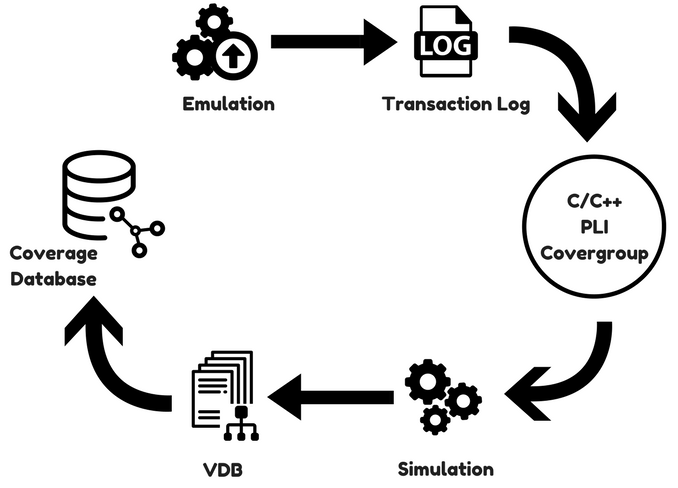
\includegraphics[scale=0.8]{./figures/coverage_collection_on_emulator.png}
\caption{Coverage collection on emulator}
\label{fig:coverage_collection_on_emulator.png}
\end{figure}

\section{C++ Language}
C++ is a general purpose programming language. It has imperative, object-oriented and generic programming features, while also providing facilities for low-level memory manipulation.
\section{VERILOG PLI}
The Verilog Programming Language Interface (Verilog PLI), is one of the more powerful features of Verilog. The PLI provides a means for both hardware designers and software engineers to interface their own programs to commercial Verilog simulators. Through this interface, a Verilog simulator can be customized to perform virtually any engineering task desired. Few common uses of the PLI include interfacing Verilog simulations to C language models, adding custom graphical tools to a simulator, reading and writing proprietary file formats from within a simulation, performing test coverage analysis during simulation etc.
\section{FUNCTIONAL COVERAGE}
Functional coverage is a user-defined metric in SystemVerilog that measures how much of the design specification, as enumerated by features in the test plan, has been exercised.\\
The key aspects of functional coverage are as follows:
\begin{itemize}
\item[-] It is user-specified and is not automatically inferred from the design.
\item[-] It is based on the design specification and is thus independent of the actual design
code or its structure.
\end{itemize}
\subsection{COVERGROUP}
The covergroup construct encapsulates the specification of a coverage model. Each covergroup specification can include the following components:
\begin{itemize}
\item[-] A clocking event that synchronizes the sampling of coverage points
\item[-] A set of coverage points
\item[-] Cross coverage between coverage points
\item[-] Optional formal arguments
\item[-] Coverage options
\end{itemize}
\subsubsection{Coverpoint}
A covergroup can contain one or more coverage points. A coverage point specifies an integral expression that is to be covered. Each coverage point includes a set of bins associated with the sampled values or value transitions of the covered expression. The bins can be explicitly defined by the user or automatically created by SystemVerilog.
